\documentclass[a4paper,11pt]{article}

\usepackage[utf8]{inputenc}
\usepackage[T1]{fontenc}
\usepackage[english]{babel}
\usepackage{color}

\usepackage{graphicx} % Inclusion d'images
\usepackage{amsfonts} % Symboles maths
\usepackage{amsmath} % Aligner les équations
\usepackage{fullpage} % Marges
\usepackage{xspace} % Espace après macros
\usepackage{float} % Positionnement des images

\title{Geometric Modelling}
\author{BLÉRON Alexandre\\MEYRON Jocelyn}
\date{January 15th, 2015}

\begin{document}

\maketitle

For each scheme, we first describe its expected properties (like the smoothness
of the limit curve), then we test it on a closed polygon and finally, we compare
the results to the expected ones.

Visually, the limit curve will be continuous if there are no holes in it, it
will be of class $ C^1 $ if the tangent is continuous and of class $ C^2 $ if
its second derivative, the curvature (which is approximated here by the list of
interior angles of the polygon) is continuous.

\section{Chaikin scheme}

The Chaikin scheme is defined by:

$$
    \begin{cases}
        x_{2i}^{n+1} = \frac{1}{4} x_{i+1}^n + \frac{3}{4} x_{i}^n \\
        x_{2i + 1}^{n+1} = \frac{3}{4} x_{i+1}^n + \frac{1}{4} x_{i}^n \\
    \end{cases}
$$

We proved, during the lecture, that the limit curve must be of class $ C^1 $.

Here is an example where we apply the Chaikin scheme on a closed polygon:

\begin{figure}[H]
\centering
\begin{minipage}{0.35\paperwidth}
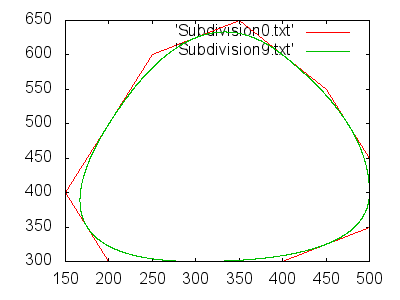
\includegraphics[scale=0.75]{pic/poly0.png}
\end{minipage}
\begin{minipage}{0.35\paperwidth}
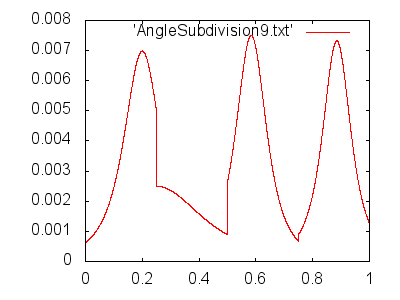
\includegraphics[scale=0.75]{pic/angle0.png}
\end{minipage}
\caption{Chaikin scheme}
\end{figure}

On the two graphs, we clearly see that the limit curve is of class $ C^1 $ .

\section{Corner cutting}
% TODO
% 2 cases: a = b + 1/2 and a /= b + 1/2

The corner cutting scheme is defined by:

$$
    \begin{cases}
        x_{2i}^{n+1} = (1 - a) x_{i+1}^n + a x_{i}^n \\
        x_{2i + 1}^{n+1} = (1 - b) x_{i+1}^n + b x_{i}^n \\
    \end{cases}
$$

We proved that if $ a = b + \frac{1}{2} $ (which is the case for the Chaikin
scheme with $ a = \frac{3}{4} $ and $ b = \frac{1}{4} $) then the limit curve
will be of class $ C^1 $. Otherwise, it is only continuous.

\begin{figure}[H]
\centering
\begin{minipage}{0.35\paperwidth}
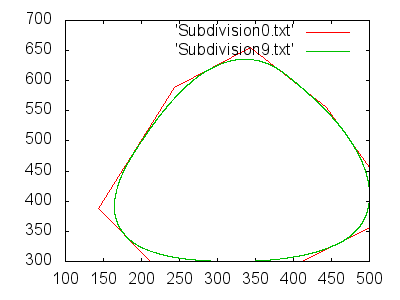
\includegraphics[scale=0.75]{pic/poly1.png}
\end{minipage}
\begin{minipage}{0.35\paperwidth}
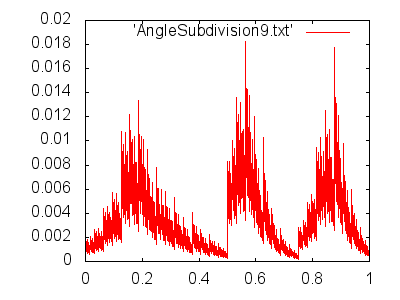
\includegraphics[scale=0.75]{pic/angle1.png}
\end{minipage}
\caption{Corner cutting scheme with $ a = 0.22 + 0.5 $ and $ b = 0.22 $}
\end{figure}

\section{Four points scheme}
% TODO

The four points scheme cutting scheme is defined by:

$$
    \begin{cases}
        x_{2i}^{n+1} = x_i^n \\
        x_{2i+1}^{n+1} = -\frac{1}{8} \frac{x_{i-1}^n + x_{i+2}^n}{2} +
        \frac{9}{8} \frac{x_i^n + x_{i+1}^n}{2} \\
    \end{cases}
$$

The limit curve must be of class $ C^1 $.

\begin{figure}[H]
\centering
\begin{minipage}{0.35\paperwidth}
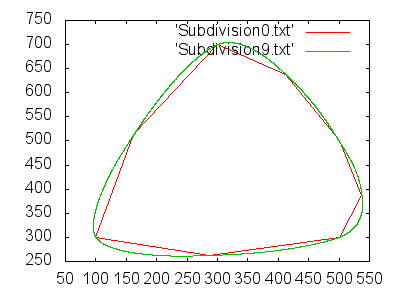
\includegraphics[scale=0.75]{pic/poly2.png}
\end{minipage}
\begin{minipage}{0.35\paperwidth}
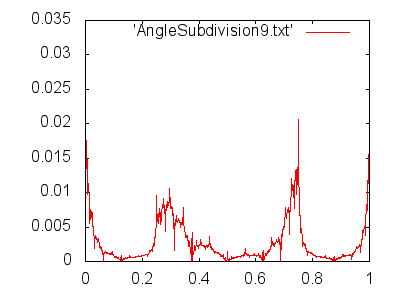
\includegraphics[scale=0.75]{pic/angle2.png}
\end{minipage}
\caption{Four points scheme}
\end{figure}

\section{Generalized four points scheme}
% TODO: test other epsilons

The generalized four points scheme cutting scheme is defined by:

$$
    \begin{cases}
        x_{2i}^{n+1} = x_i^n \\
        x_{2i+1}^{n+1} = -\epsilon \frac{x_{i-1}^n + x_{i+2}^n}{2} +
        (1 + \epsilon) \frac{x_i^n + x_{i+1}^n}{2} \\
    \end{cases}
$$

There exists a value of $ \epsilon $ for which the limit curve if of class $ C^1
$.

\begin{figure}[H]
\centering
\begin{minipage}{0.35\paperwidth}
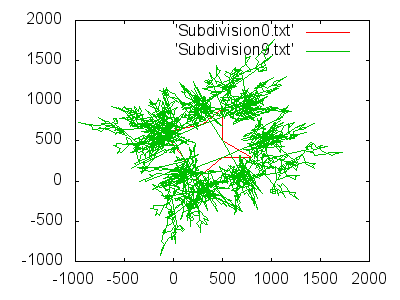
\includegraphics[scale=0.75]{pic/poly3.png}
\end{minipage}
\begin{minipage}{0.35\paperwidth}
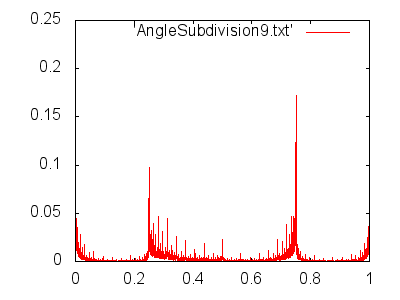
\includegraphics[scale=0.75]{pic/angle3.png}
\end{minipage}
\caption{Generalized four points scheme with $ \epsilon = 0.1 $}
\end{figure}

\section{Uniform splines of degree 3}
% TODO

The uniform splines of degree $ k $ scheme is defined by:
\begin{enumerate}
    \item Duplication: construct $ (d_i^0) $ such that: $ d_{2i}^n = x_i^n $ and
        $ d_{2i+1}^n = x_i^n $.
    \item $ k $ steps of averaging : $ d_i^{j+1} = \frac{d_i^j +d_{i+1}^j}{2} $.
    \item The result is the sequence $ (d_i^k) $.
\end{enumerate}

\begin{figure}[H]
\centering
\begin{minipage}{0.35\paperwidth}
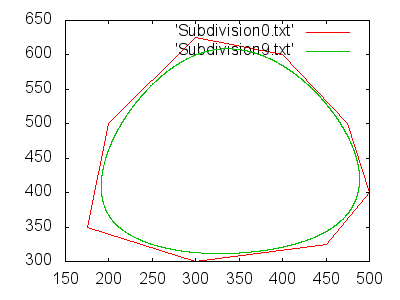
\includegraphics[scale=0.75]{pic/poly4.png}
\end{minipage}
\begin{minipage}{0.35\paperwidth}
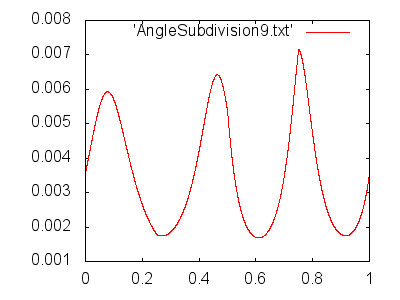
\includegraphics[scale=0.75]{pic/angle4.png}
\end{minipage}
\caption{Uniform splines of degree 3}
\end{figure}

\end{document}

